\documentclass[1p]{elsarticle_modified}
%\bibliographystyle{elsarticle-num}

%\usepackage[colorlinks]{hyperref}
%\usepackage{abbrmath_seonhwa} %\Abb, \Ascr, \Acal ,\Abf, \Afrak
\usepackage{amsfonts}
\usepackage{amssymb}
\usepackage{amsmath}
\usepackage{amsthm}
\usepackage{scalefnt}
\usepackage{amsbsy}
\usepackage{kotex}
\usepackage{caption}
\usepackage{subfig}
\usepackage{color}
\usepackage{graphicx}
\usepackage{xcolor} %% white, black, red, green, blue, cyan, magenta, yellow
\usepackage{float}
\usepackage{setspace}
\usepackage{hyperref}

\usepackage{tikz}
\usetikzlibrary{arrows}

\usepackage{multirow}
\usepackage{array} % fixed length table
\usepackage{hhline}

%%%%%%%%%%%%%%%%%%%%%
\makeatletter
\renewcommand*\env@matrix[1][\arraystretch]{%
	\edef\arraystretch{#1}%
	\hskip -\arraycolsep
	\let\@ifnextchar\new@ifnextchar
	\array{*\c@MaxMatrixCols c}}
\makeatother %https://tex.stackexchange.com/questions/14071/how-can-i-increase-the-line-spacing-in-a-matrix
%%%%%%%%%%%%%%%

\usepackage[normalem]{ulem}

\newcommand{\msout}[1]{\ifmmode\text{\sout{\ensuremath{#1}}}\else\sout{#1}\fi}
%SOURCE: \msout is \stkout macro in https://tex.stackexchange.com/questions/20609/strikeout-in-math-mode

\newcommand{\cancel}[1]{
	\ifmmode
	{\color{red}\msout{#1}}
	\else
	{\color{red}\sout{#1}}
	\fi
}

\newcommand{\add}[1]{
	{\color{blue}\uwave{#1}}
}

\newcommand{\replace}[2]{
	\ifmmode
	{\color{red}\msout{#1}}{\color{blue}\uwave{#2}}
	\else
	{\color{red}\sout{#1}}{\color{blue}\uwave{#2}}
	\fi
}

\newcommand{\Sol}{\mathcal{S}} %segment
\newcommand{\D}{D} %diagram
\newcommand{\A}{\mathcal{A}} %arc


%%%%%%%%%%%%%%%%%%%%%%%%%%%%%5 test

\def\sl{\operatorname{\textup{SL}}(2,\Cbb)}
\def\psl{\operatorname{\textup{PSL}}(2,\Cbb)}
\def\quan{\mkern 1mu \triangleright \mkern 1mu}

\theoremstyle{definition}
\newtheorem{thm}{Theorem}[section]
\newtheorem{prop}[thm]{Proposition}
\newtheorem{lem}[thm]{Lemma}
\newtheorem{ques}[thm]{Question}
\newtheorem{cor}[thm]{Corollary}
\newtheorem{defn}[thm]{Definition}
\newtheorem{exam}[thm]{Example}
\newtheorem{rmk}[thm]{Remark}
\newtheorem{alg}[thm]{Algorithm}

\newcommand{\I}{\sqrt{-1}}
\begin{document}

%\begin{frontmatter}
%
%\title{Boundary parabolic representations of knots up to 8 crossings}
%
%%% Group authors per affiliation:
%\author{Yunhi Cho} 
%\address{Department of Mathematics, University of Seoul, Seoul, Korea}
%\ead{yhcho@uos.ac.kr}
%
%
%\author{Seonhwa Kim} %\fnref{s_kim}}
%\address{Center for Geometry and Physics, Institute for Basic Science, Pohang, 37673, Korea}
%\ead{ryeona17@ibs.re.kr}
%
%\author{Hyuk Kim}
%\address{Department of Mathematical Sciences, Seoul National University, Seoul 08826, Korea}
%\ead{hyukkim@snu.ac.kr}
%
%\author{Seokbeom Yoon}
%\address{Department of Mathematical Sciences, Seoul National University, Seoul, 08826,  Korea}
%\ead{sbyoon15@snu.ac.kr}
%
%\begin{abstract}
%We find all boundary parabolic representation of knots up to 8 crossings.
%
%\end{abstract}
%\begin{keyword}
%    \MSC[2010] 57M25 
%\end{keyword}
%
%\end{frontmatter}

%\linenumbers
%\tableofcontents
%
\newcommand\colored[1]{\textcolor{white}{\rule[-0.35ex]{0.8em}{1.4ex}}\kern-0.8em\color{red} #1}%
%\newcommand\colored[1]{\textcolor{white}{ #1}\kern-2.17ex	\textcolor{white}{ #1}\kern-1.81ex	\textcolor{white}{ #1}\kern-2.15ex\color{red}#1	}

{\Large $\underline{12a_{1046}~(K12a_{1046})}$}

\setlength{\tabcolsep}{10pt}
\renewcommand{\arraystretch}{1.6}
\vspace{1cm}\begin{tabular}{m{100pt}>{\centering\arraybackslash}m{274pt}}
\multirow{5}{120pt}{
	\centering
	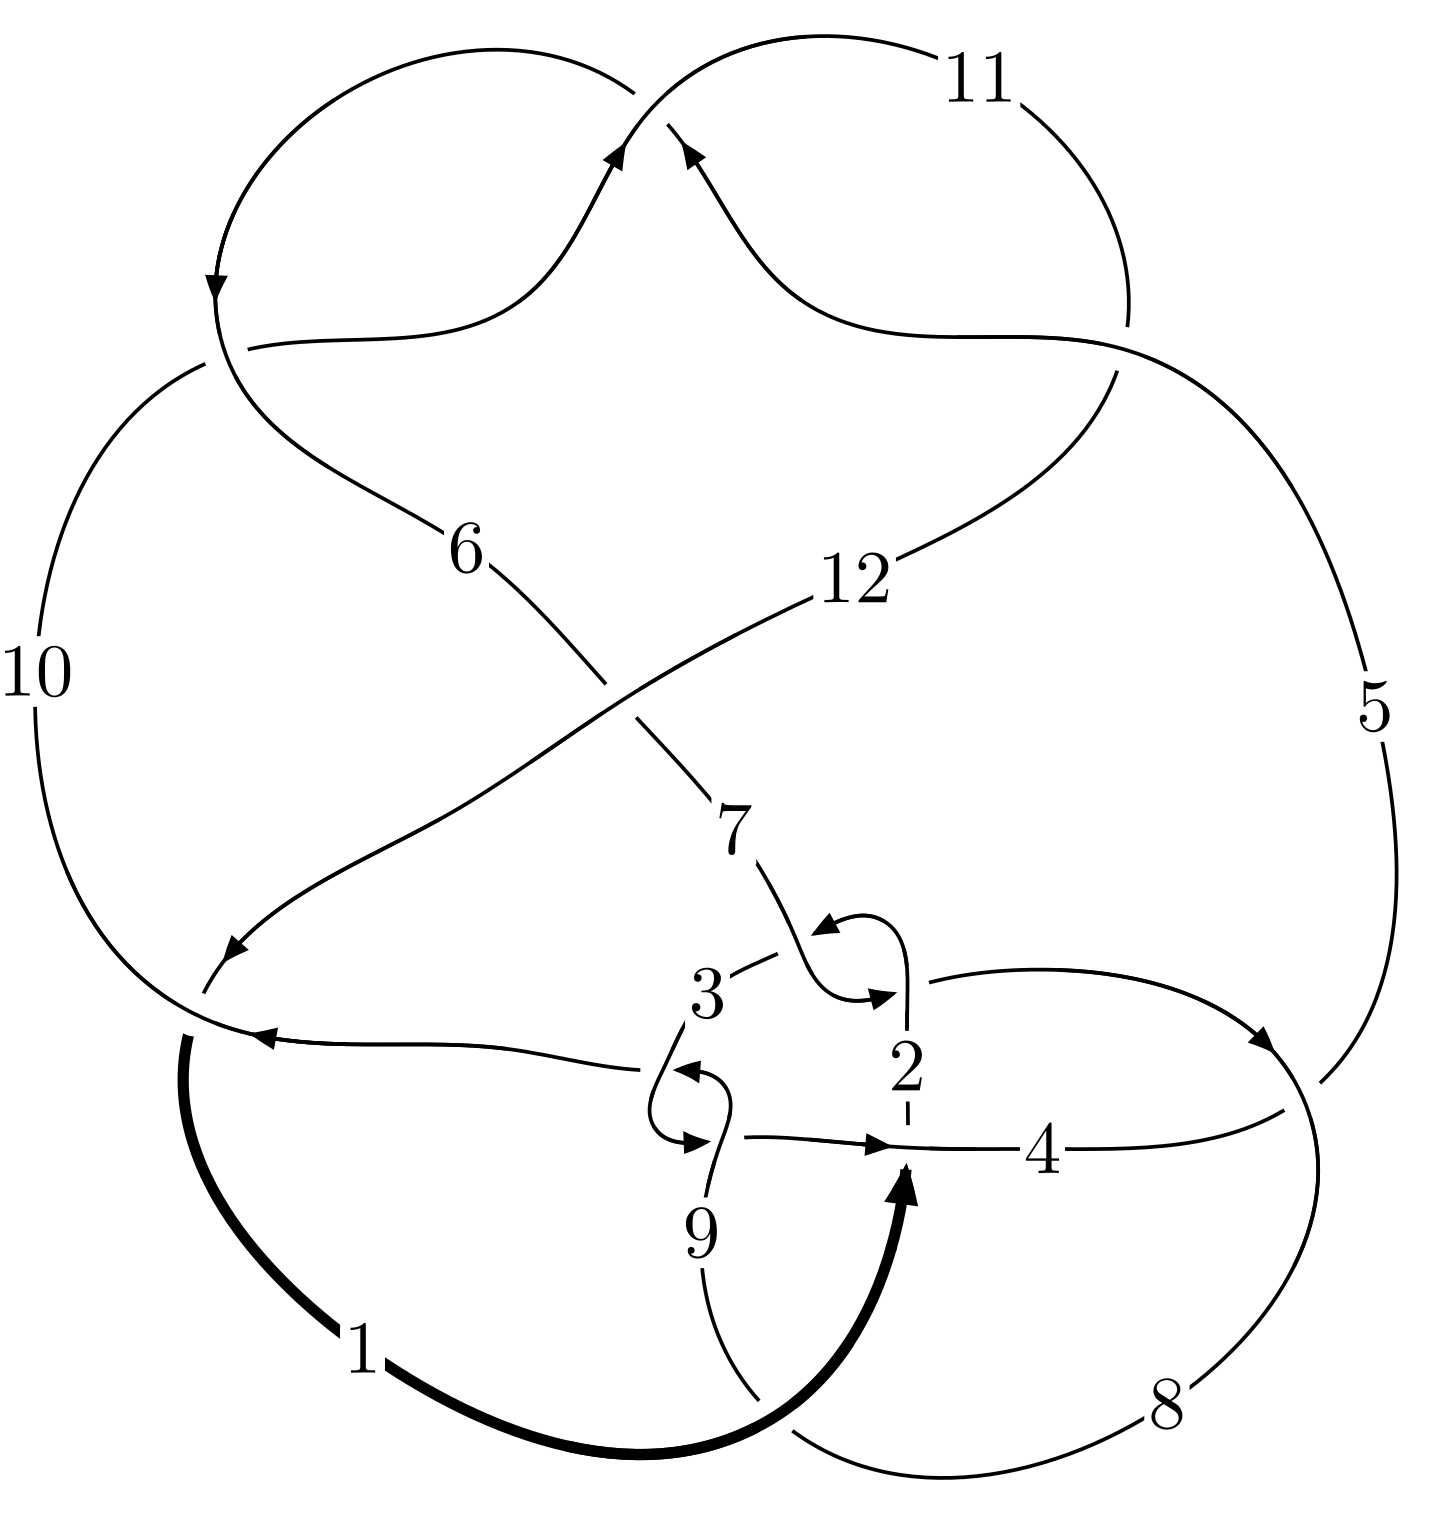
\includegraphics[width=112pt]{../../../GIT/diagram.site/Diagrams/png/1847_12a_1046.png}\\
\ \ \ A knot diagram\footnotemark}&
\allowdisplaybreaks
\textbf{Linearized knot diagam} \\
\cline{2-2}
 &
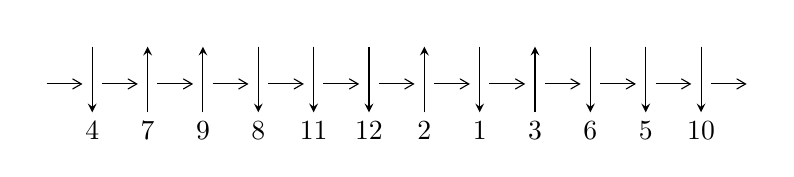
\begin{tikzpicture}[x=20pt, y=17pt]
	% nodes
	\node (C0) at (0, 0) {};
	\node (C1) at (1, 0) {};
	\node (C1U) at (1, +1) {};
	\node (C1D) at (1, -1) {4};

	\node (C2) at (2, 0) {};
	\node (C2U) at (2, +1) {};
	\node (C2D) at (2, -1) {7};

	\node (C3) at (3, 0) {};
	\node (C3U) at (3, +1) {};
	\node (C3D) at (3, -1) {9};

	\node (C4) at (4, 0) {};
	\node (C4U) at (4, +1) {};
	\node (C4D) at (4, -1) {8};

	\node (C5) at (5, 0) {};
	\node (C5U) at (5, +1) {};
	\node (C5D) at (5, -1) {11};

	\node (C6) at (6, 0) {};
	\node (C6U) at (6, +1) {};
	\node (C6D) at (6, -1) {12};

	\node (C7) at (7, 0) {};
	\node (C7U) at (7, +1) {};
	\node (C7D) at (7, -1) {2};

	\node (C8) at (8, 0) {};
	\node (C8U) at (8, +1) {};
	\node (C8D) at (8, -1) {1};

	\node (C9) at (9, 0) {};
	\node (C9U) at (9, +1) {};
	\node (C9D) at (9, -1) {3};

	\node (C10) at (10, 0) {};
	\node (C10U) at (10, +1) {};
	\node (C10D) at (10, -1) {6};

	\node (C11) at (11, 0) {};
	\node (C11U) at (11, +1) {};
	\node (C11D) at (11, -1) {5};

	\node (C12) at (12, 0) {};
	\node (C12U) at (12, +1) {};
	\node (C12D) at (12, -1) {10};
	\node (C13) at (13, 0) {};

	% arrows
	\draw[->,>={angle 60}]
	(C0) edge (C1) (C1) edge (C2) (C2) edge (C3) (C3) edge (C4) (C4) edge (C5) (C5) edge (C6) (C6) edge (C7) (C7) edge (C8) (C8) edge (C9) (C9) edge (C10) (C10) edge (C11) (C11) edge (C12) (C12) edge (C13) ;	\draw[->,>=stealth]
	(C1U) edge (C1D) (C2D) edge (C2U) (C3D) edge (C3U) (C4U) edge (C4D) (C5U) edge (C5D) (C6U) edge (C6D) (C7D) edge (C7U) (C8U) edge (C8D) (C9D) edge (C9U) (C10U) edge (C10D) (C11U) edge (C11D) (C12U) edge (C12D) ;
	\end{tikzpicture} \\
\hhline{~~} \\& 
\textbf{Solving Sequence} \\ \cline{2-2} 
 &
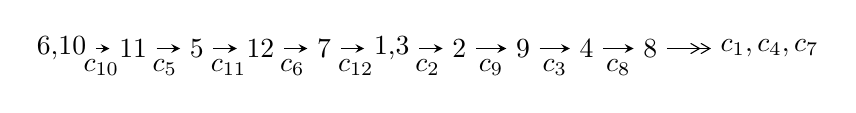
\begin{tikzpicture}[x=23pt, y=7pt]
	% node
	\node (A0) at (-1/8, 0) {6,10};
	\node (A1) at (1, 0) {11};
	\node (A2) at (2, 0) {5};
	\node (A3) at (3, 0) {12};
	\node (A4) at (4, 0) {7};
	\node (A5) at (81/16, 0) {1,3};
	\node (A6) at (49/8, 0) {2};
	\node (A7) at (57/8, 0) {9};
	\node (A8) at (65/8, 0) {4};
	\node (A9) at (73/8, 0) {8};
	\node (C1) at (1/2, -1) {$c_{10}$};
	\node (C2) at (3/2, -1) {$c_{5}$};
	\node (C3) at (5/2, -1) {$c_{11}$};
	\node (C4) at (7/2, -1) {$c_{6}$};
	\node (C5) at (9/2, -1) {$c_{12}$};
	\node (C6) at (45/8, -1) {$c_{2}$};
	\node (C7) at (53/8, -1) {$c_{9}$};
	\node (C8) at (61/8, -1) {$c_{3}$};
	\node (C9) at (69/8, -1) {$c_{8}$};
	\node (A10) at (11, 0) {$c_{1},c_{4},c_{7}$};

	% edge
	\draw[->,>=stealth]	
	(A0) edge (A1) (A1) edge (A2) (A2) edge (A3) (A3) edge (A4) (A4) edge (A5) (A5) edge (A6) (A6) edge (A7) (A7) edge (A8) (A8) edge (A9) ;
	\draw[->>,>={angle 60}]	
	(A9) edge (A10);
\end{tikzpicture} \\ 

\end{tabular} \\

\footnotetext{
The image of knot diagram is generated by the software ``\textbf{Draw programme}" developed by Andrew Bartholomew(\url{http://www.layer8.co.uk/maths/draw/index.htm\#Running-draw}), where we modified some parts for our purpose(\url{https://github.com/CATsTAILs/LinksPainter}).
}\phantom \\ \newline 
\centering \textbf{Ideals for irreducible components\footnotemark of $X_{\text{par}}$} 
 
\begin{align*}
I^u_{1}&=\langle 
17 u^{38}+107 u^{37}+\cdots+4 b-260,\;21 u^{38}+133 u^{37}+\cdots+8 a-60,\;u^{39}+7 u^{38}+\cdots-60 u-8\rangle \\
I^u_{2}&=\langle 
6.66973\times10^{28} a^{5} u^{13}+1.23560\times10^{29} a^{4} u^{13}+\cdots-4.72555\times10^{29} a+3.07955\times10^{29},\\
\phantom{I^u_{2}}&\phantom{= \langle  }2 u^{13} a^4+7 u^{13} a^3+\cdots-6 a-15,\\
\phantom{I^u_{2}}&\phantom{= \langle  }u^{14}- u^{13}+7 u^{12}-6 u^{11}+18 u^{10}-13 u^9+19 u^8-10 u^7+4 u^6+2 u^5-4 u^4+4 u^3- u+1\rangle \\
I^u_{3}&=\langle 
- u^{17}-8 u^{15}-25 u^{13}-37 u^{11}- u^{10}-25 u^9-5 u^8-8 u^7-8 u^6-6 u^5-3 u^4-4 u^3+2 u^2+b- u,\\
\phantom{I^u_{3}}&\phantom{= \langle  }u^{21}+u^{20}+\cdots+a+1,\;u^{22}+11 u^{20}+\cdots+2 u+1\rangle \\
\\
\end{align*}
\raggedright * 3 irreducible components of $\dim_{\mathbb{C}}=0$, with total 145 representations.\\
\footnotetext{All coefficients of polynomials are rational numbers. But the coefficients are sometimes approximated in decimal forms when there is not enough margin.}
\newpage
\renewcommand{\arraystretch}{1}
\centering \section*{I. $I^u_{1}= \langle 17 u^{38}+107 u^{37}+\cdots+4 b-260,\;21 u^{38}+133 u^{37}+\cdots+8 a-60,\;u^{39}+7 u^{38}+\cdots-60 u-8 \rangle$}
\flushleft \textbf{(i) Arc colorings}\\
\begin{tabular}{m{7pt} m{180pt} m{7pt} m{180pt} }
\flushright $a_{6}=$&$\begin{pmatrix}0\\u\end{pmatrix}$ \\
\flushright $a_{10}=$&$\begin{pmatrix}1\\0\end{pmatrix}$ \\
\flushright $a_{11}=$&$\begin{pmatrix}1\\u^2\end{pmatrix}$ \\
\flushright $a_{5}=$&$\begin{pmatrix}u\\u^3+u\end{pmatrix}$ \\
\flushright $a_{12}=$&$\begin{pmatrix}u^2+1\\u^4+2 u^2\end{pmatrix}$ \\
\flushright $a_{7}=$&$\begin{pmatrix}- u^5-2 u^3- u\\- u^7-3 u^5-2 u^3+u\end{pmatrix}$ \\
\flushright $a_{1}=$&$\begin{pmatrix}- u^4- u^2+1\\u^4+2 u^2\end{pmatrix}$ \\
\flushright $a_{3}=$&$\begin{pmatrix}-2.62500 u^{38}-16.6250 u^{37}+\cdots+105.750 u+7.50000\\-\frac{17}{4} u^{38}-\frac{107}{4} u^{37}+\cdots+388 u+65\end{pmatrix}$ \\
\flushright $a_{2}=$&$\begin{pmatrix}2.37500 u^{38}+18.3750 u^{37}+\cdots-176.250 u-22.5000\\\frac{11}{4} u^{38}+\frac{57}{4} u^{37}+\cdots-210 u-33\end{pmatrix}$ \\
\flushright $a_{9}=$&$\begin{pmatrix}-\frac{55}{8} u^{38}-\frac{371}{8} u^{37}+\cdots+\frac{1737}{4} u+66\\\frac{17}{4} u^{38}+\frac{105}{4} u^{37}+\cdots-\frac{243}{2} u-13\end{pmatrix}$ \\
\flushright $a_{4}=$&$\begin{pmatrix}-\frac{29}{8} u^{38}-\frac{207}{8} u^{37}+\cdots+\frac{421}{2} u+24\\-4 u^{38}-\frac{47}{2} u^{37}+\cdots+\frac{747}{2} u+61\end{pmatrix}$ \\
\flushright $a_{8}=$&$\begin{pmatrix}-\frac{13}{8} u^{38}-\frac{65}{8} u^{37}+\cdots+\frac{3}{4} u+1\\-\frac{19}{4} u^{38}-\frac{127}{4} u^{37}+\cdots+\frac{661}{2} u+51\end{pmatrix}$\\&\end{tabular}
\flushleft \textbf{(ii) Obstruction class $= -1$}\\~\\
\flushleft \textbf{(iii) Cusp Shapes $= 6 u^{38}+36 u^{37}+\cdots-148 u-10$}\\~\\
\newpage\renewcommand{\arraystretch}{1}
\flushleft \textbf{(iv) u-Polynomials at the component}\newline \\
\begin{tabular}{m{50pt}|m{274pt}}
Crossings & \hspace{64pt}u-Polynomials at each crossing \\
\hline $$\begin{aligned}c_{1}\end{aligned}$$&$\begin{aligned}
&u^{39}-33 u^{38}+\cdots+352256 u-16384
\end{aligned}$\\
\hline $$\begin{aligned}c_{2},c_{3},c_{7}\\c_{9}\end{aligned}$$&$\begin{aligned}
&u^{39}+13 u^{37}+\cdots-2 u+1
\end{aligned}$\\
\hline $$\begin{aligned}c_{4},c_{8}\end{aligned}$$&$\begin{aligned}
&u^{39}+u^{38}+\cdots+3 u+1
\end{aligned}$\\
\hline $$\begin{aligned}c_{5},c_{10},c_{11}\end{aligned}$$&$\begin{aligned}
&u^{39}-7 u^{38}+\cdots-60 u+8
\end{aligned}$\\
\hline $$\begin{aligned}c_{6}\end{aligned}$$&$\begin{aligned}
&u^{39}+7 u^{38}+\cdots-1596 u+2088
\end{aligned}$\\
\hline $$\begin{aligned}c_{12}\end{aligned}$$&$\begin{aligned}
&u^{39}-9 u^{38}+\cdots-43968 u+9728
\end{aligned}$\\
\hline
\end{tabular}\\~\\
\newpage\renewcommand{\arraystretch}{1}
\flushleft \textbf{(v) Riley Polynomials at the component}\newline \\
\begin{tabular}{m{50pt}|m{274pt}}
Crossings & \hspace{64pt}Riley Polynomials at each crossing \\
\hline $$\begin{aligned}c_{1}\end{aligned}$$&$\begin{aligned}
&y^{39}-9 y^{38}+\cdots+3019898880 y-268435456
\end{aligned}$\\
\hline $$\begin{aligned}c_{2},c_{3},c_{7}\\c_{9}\end{aligned}$$&$\begin{aligned}
&y^{39}+26 y^{38}+\cdots+8 y-1
\end{aligned}$\\
\hline $$\begin{aligned}c_{4},c_{8}\end{aligned}$$&$\begin{aligned}
&y^{39}+9 y^{38}+\cdots-23 y-1
\end{aligned}$\\
\hline $$\begin{aligned}c_{5},c_{10},c_{11}\end{aligned}$$&$\begin{aligned}
&y^{39}+35 y^{38}+\cdots-48 y-64
\end{aligned}$\\
\hline $$\begin{aligned}c_{6}\end{aligned}$$&$\begin{aligned}
&y^{39}+5 y^{38}+\cdots-35220528 y-4359744
\end{aligned}$\\
\hline $$\begin{aligned}c_{12}\end{aligned}$$&$\begin{aligned}
&y^{39}+15 y^{38}+\cdots-1741041664 y-94633984
\end{aligned}$\\
\hline
\end{tabular}\\~\\
\newpage\flushleft \textbf{(vi) Complex Volumes and Cusp Shapes}
$$\begin{array}{c|c|c}  
\text{Solutions to }I^u_{1}& \I (\text{vol} + \sqrt{-1}CS) & \text{Cusp shape}\\
 \hline 
\begin{aligned}
u &= -0.402641 + 0.923218 I \\
a &= \phantom{-}0.123865 + 0.173423 I \\
b &= -0.313293 + 0.898902 I\end{aligned}
 & -0.83222 - 1.74805 I & \phantom{-}1.85163 + 7.08327 I \\ \hline\begin{aligned}
u &= -0.402641 - 0.923218 I \\
a &= \phantom{-}0.123865 - 0.173423 I \\
b &= -0.313293 - 0.898902 I\end{aligned}
 & -0.83222 + 1.74805 I & \phantom{-}1.85163 - 7.08327 I \\ \hline\begin{aligned}
u &= -0.711880 + 0.543145 I \\
a &= -0.596131 - 0.139383 I \\
b &= \phantom{-}0.047860 + 0.975188 I\end{aligned}
 & -0.45441 + 2.42357 I & -6.62342 - 4.26652 I \\ \hline\begin{aligned}
u &= -0.711880 - 0.543145 I \\
a &= -0.596131 + 0.139383 I \\
b &= \phantom{-}0.047860 - 0.975188 I\end{aligned}
 & -0.45441 - 2.42357 I & -6.62342 + 4.26652 I \\ \hline\begin{aligned}
u &= -0.477289 + 0.710961 I \\
a &= -0.147405 + 0.420958 I \\
b &= \phantom{-}0.54795 - 1.36232 I\end{aligned}
 & -4.43014 - 10.11780 I & -6.08524 + 4.54583 I \\ \hline\begin{aligned}
u &= -0.477289 - 0.710961 I \\
a &= -0.147405 - 0.420958 I \\
b &= \phantom{-}0.54795 + 1.36232 I\end{aligned}
 & -4.43014 + 10.11780 I & -6.08524 - 4.54583 I \\ \hline\begin{aligned}
u &= -0.790989 + 0.257645 I \\
a &= -1.01138 + 1.09144 I \\
b &= \phantom{-}0.403002 + 0.993100 I\end{aligned}
 & -2.87677 + 6.11596 I & -5.61902 - 11.75200 I \\ \hline\begin{aligned}
u &= -0.790989 - 0.257645 I \\
a &= -1.01138 - 1.09144 I \\
b &= \phantom{-}0.403002 - 0.993100 I\end{aligned}
 & -2.87677 - 6.11596 I & -5.61902 + 11.75200 I \\ \hline\begin{aligned}
u &= \phantom{-}0.342776 + 1.125240 I \\
a &= -1.077400 - 0.136141 I \\
b &= \phantom{-}0.39377 - 1.36577 I\end{aligned}
 & -5.82056 - 9.89475 I & -7.41952 + 7.73819 I \\ \hline\begin{aligned}
u &= \phantom{-}0.342776 - 1.125240 I \\
a &= -1.077400 + 0.136141 I \\
b &= \phantom{-}0.39377 + 1.36577 I\end{aligned}
 & -5.82056 + 9.89475 I & -7.41952 - 7.73819 I\\
 \hline 
 \end{array}$$\newpage$$\begin{array}{c|c|c}  
\text{Solutions to }I^u_{1}& \I (\text{vol} + \sqrt{-1}CS) & \text{Cusp shape}\\
 \hline 
\begin{aligned}
u &= -0.755894 + 0.317559 I \\
a &= \phantom{-}1.61018 - 1.04698 I \\
b &= -0.59395 - 1.40684 I\end{aligned}
 & -5.7809 + 14.4369 I & -8.07183 - 9.36551 I \\ \hline\begin{aligned}
u &= -0.755894 - 0.317559 I \\
a &= \phantom{-}1.61018 + 1.04698 I \\
b &= -0.59395 + 1.40684 I\end{aligned}
 & -5.7809 - 14.4369 I & -8.07183 + 9.36551 I \\ \hline\begin{aligned}
u &= \phantom{-}0.798444 + 0.067462 I \\
a &= -0.366765 - 1.043450 I \\
b &= -0.305676 - 1.327300 I\end{aligned}
 & -9.06750 + 5.75506 I & -11.48705 - 4.63489 I \\ \hline\begin{aligned}
u &= \phantom{-}0.798444 - 0.067462 I \\
a &= -0.366765 + 1.043450 I \\
b &= -0.305676 + 1.327300 I\end{aligned}
 & -9.06750 - 5.75506 I & -11.48705 + 4.63489 I \\ \hline\begin{aligned}
u &= -0.624159 + 0.368707 I \\
a &= -0.309607 + 0.944919 I \\
b &= \phantom{-}0.742260 - 0.072896 I\end{aligned}
 & \phantom{-}2.43896 + 3.63567 I & \phantom{-}0.57871 - 5.66121 I \\ \hline\begin{aligned}
u &= -0.624159 - 0.368707 I \\
a &= -0.309607 - 0.944919 I \\
b &= \phantom{-}0.742260 + 0.072896 I\end{aligned}
 & \phantom{-}2.43896 - 3.63567 I & \phantom{-}0.57871 + 5.66121 I \\ \hline\begin{aligned}
u &= \phantom{-}0.141393 + 1.269230 I \\
a &= \phantom{-}0.171501 + 0.444677 I \\
b &= -0.487698 - 0.033283 I\end{aligned}
 & \phantom{-}2.67445 - 2.43754 I & \phantom{-0.000000 } 0 \\ \hline\begin{aligned}
u &= \phantom{-}0.141393 - 1.269230 I \\
a &= \phantom{-}0.171501 - 0.444677 I \\
b &= -0.487698 + 0.033283 I\end{aligned}
 & \phantom{-}2.67445 + 2.43754 I & \phantom{-0.000000 } 0 \\ \hline\begin{aligned}
u &= \phantom{-}0.359384 + 1.271690 I \\
a &= \phantom{-}0.786179 - 0.431294 I \\
b &= \phantom{-}0.228282 + 1.275960 I\end{aligned}
 & -4.91124 + 1.59162 I & \phantom{-0.000000 } 0 \\ \hline\begin{aligned}
u &= \phantom{-}0.359384 - 1.271690 I \\
a &= \phantom{-}0.786179 + 0.431294 I \\
b &= \phantom{-}0.228282 - 1.275960 I\end{aligned}
 & -4.91124 - 1.59162 I & \phantom{-0.000000 } 0\\
 \hline 
 \end{array}$$\newpage$$\begin{array}{c|c|c}  
\text{Solutions to }I^u_{1}& \I (\text{vol} + \sqrt{-1}CS) & \text{Cusp shape}\\
 \hline 
\begin{aligned}
u &= -0.513565 + 0.443254 I \\
a &= \phantom{-}0.813961 - 0.283065 I \\
b &= -0.740571 - 0.193624 I\end{aligned}
 & \phantom{-}2.83998 + 0.06866 I & \phantom{-}1.72690 - 2.02626 I \\ \hline\begin{aligned}
u &= -0.513565 - 0.443254 I \\
a &= \phantom{-}0.813961 + 0.283065 I \\
b &= -0.740571 + 0.193624 I\end{aligned}
 & \phantom{-}2.83998 - 0.06866 I & \phantom{-}1.72690 + 2.02626 I \\ \hline\begin{aligned}
u &= \phantom{-}0.286826 + 0.574932 I \\
a &= \phantom{-}0.705124 + 0.432129 I \\
b &= -0.204549 + 0.657112 I\end{aligned}
 & -0.221784 - 1.394250 I & -2.01573 + 3.25063 I \\ \hline\begin{aligned}
u &= \phantom{-}0.286826 - 0.574932 I \\
a &= \phantom{-}0.705124 - 0.432129 I \\
b &= -0.204549 - 0.657112 I\end{aligned}
 & -0.221784 + 1.394250 I & -2.01573 - 3.25063 I \\ \hline\begin{aligned}
u &= -0.06245 + 1.42153 I \\
a &= -1.195630 + 0.599024 I \\
b &= \phantom{-}0.571644 - 0.706847 I\end{aligned}
 & \phantom{-}6.09815 - 1.32183 I & \phantom{-0.000000 } 0 \\ \hline\begin{aligned}
u &= -0.06245 - 1.42153 I \\
a &= -1.195630 - 0.599024 I \\
b &= \phantom{-}0.571644 + 0.706847 I\end{aligned}
 & \phantom{-}6.09815 + 1.32183 I & \phantom{-0.000000 } 0 \\ \hline\begin{aligned}
u &= -0.31542 + 1.41590 I \\
a &= \phantom{-}1.78095 - 0.15255 I \\
b &= -0.470372 - 1.030310 I\end{aligned}
 & \phantom{-}2.46313 + 10.11530 I & \phantom{-0.000000 } 0 \\ \hline\begin{aligned}
u &= -0.31542 - 1.41590 I \\
a &= \phantom{-}1.78095 + 0.15255 I \\
b &= -0.470372 + 1.030310 I\end{aligned}
 & \phantom{-}2.46313 - 10.11530 I & \phantom{-0.000000 } 0 \\ \hline\begin{aligned}
u &= -0.19256 + 1.44129 I \\
a &= -1.64680 + 0.08898 I \\
b &= \phantom{-}0.847538 + 0.236025 I\end{aligned}
 & \phantom{-}8.83636 + 2.66799 I & \phantom{-0.000000 } 0 \\ \hline\begin{aligned}
u &= -0.19256 - 1.44129 I \\
a &= -1.64680 - 0.08898 I \\
b &= \phantom{-}0.847538 - 0.236025 I\end{aligned}
 & \phantom{-}8.83636 - 2.66799 I & \phantom{-0.000000 } 0\\
 \hline 
 \end{array}$$\newpage$$\begin{array}{c|c|c}  
\text{Solutions to }I^u_{1}& \I (\text{vol} + \sqrt{-1}CS) & \text{Cusp shape}\\
 \hline 
\begin{aligned}
u &= -0.23418 + 1.44082 I \\
a &= \phantom{-}1.16879 - 0.89698 I \\
b &= -0.802572 + 0.020537 I\end{aligned}
 & \phantom{-}8.24829 + 6.77910 I & \phantom{-0.000000 } 0 \\ \hline\begin{aligned}
u &= -0.23418 - 1.44082 I \\
a &= \phantom{-}1.16879 + 0.89698 I \\
b &= -0.802572 - 0.020537 I\end{aligned}
 & \phantom{-}8.24829 - 6.77910 I & \phantom{-0.000000 } 0 \\ \hline\begin{aligned}
u &= -0.29621 + 1.43559 I \\
a &= -2.41476 - 0.26767 I \\
b &= \phantom{-}0.63351 + 1.41710 I\end{aligned}
 & -0.1721 + 18.2585 I & \phantom{-0.000000 } 0 \\ \hline\begin{aligned}
u &= -0.29621 - 1.43559 I \\
a &= -2.41476 + 0.26767 I \\
b &= \phantom{-}0.63351 - 1.41710 I\end{aligned}
 & -0.1721 - 18.2585 I & \phantom{-0.000000 } 0 \\ \hline\begin{aligned}
u &= \phantom{-}0.534008\phantom{ +0.000000I} \\
a &= \phantom{-}0.570035\phantom{ +0.000000I} \\
b &= \phantom{-}0.419240\phantom{ +0.000000I}\end{aligned}
 & -1.19215\phantom{ +0.000000I} & -7.70730\phantom{ +0.000000I} \\ \hline\begin{aligned}
u &= -0.09732 + 1.48612 I \\
a &= \phantom{-}0.92868 - 1.50124 I \\
b &= -0.583941 + 1.263340 I\end{aligned}
 & \phantom{-}2.68660 - 8.37607 I & \phantom{-0.000000 } 0 \\ \hline\begin{aligned}
u &= -0.09732 - 1.48612 I \\
a &= \phantom{-}0.92868 + 1.50124 I \\
b &= -0.583941 - 1.263340 I\end{aligned}
 & \phantom{-}2.68660 + 8.37607 I & \phantom{-0.000000 } 0 \\ \hline\begin{aligned}
u &= -0.22127 + 1.51243 I \\
a &= \phantom{-}0.641621 + 0.918434 I \\
b &= -0.122823 - 0.904781 I\end{aligned}
 & \phantom{-}6.27991 + 5.75991 I & \phantom{-0.000000 } 0 \\ \hline\begin{aligned}
u &= -0.22127 - 1.51243 I \\
a &= \phantom{-}0.641621 - 0.918434 I \\
b &= -0.122823 + 0.904781 I\end{aligned}
 & \phantom{-}6.27991 - 5.75991 I & \phantom{-0.000000 } 0\\
 \hline 
 \end{array}$$\newpage\newpage\renewcommand{\arraystretch}{1}
\centering \section*{II. $I^u_{2}= \langle 6.67\times10^{28} a^{5} u^{13}+1.24\times10^{29} a^{4} u^{13}+\cdots-4.73\times10^{29} a+3.08\times10^{29},\;2 u^{13} a^4+7 u^{13} a^3+\cdots-6 a-15,\;u^{14}- u^{13}+\cdots- u+1 \rangle$}
\flushleft \textbf{(i) Arc colorings}\\
\begin{tabular}{m{7pt} m{180pt} m{7pt} m{180pt} }
\flushright $a_{6}=$&$\begin{pmatrix}0\\u\end{pmatrix}$ \\
\flushright $a_{10}=$&$\begin{pmatrix}1\\0\end{pmatrix}$ \\
\flushright $a_{11}=$&$\begin{pmatrix}1\\u^2\end{pmatrix}$ \\
\flushright $a_{5}=$&$\begin{pmatrix}u\\u^3+u\end{pmatrix}$ \\
\flushright $a_{12}=$&$\begin{pmatrix}u^2+1\\u^4+2 u^2\end{pmatrix}$ \\
\flushright $a_{7}=$&$\begin{pmatrix}- u^5-2 u^3- u\\- u^7-3 u^5-2 u^3+u\end{pmatrix}$ \\
\flushright $a_{1}=$&$\begin{pmatrix}- u^4- u^2+1\\u^4+2 u^2\end{pmatrix}$ \\
\flushright $a_{3}=$&$\begin{pmatrix}a\\-0.245209 a^{5} u^{13}-0.454264 a^{4} u^{13}+\cdots+1.73733 a-1.13218\end{pmatrix}$ \\
\flushright $a_{2}=$&$\begin{pmatrix}-0.244193 a^{5} u^{13}-0.0145692 a^{4} u^{13}+\cdots+1.26898 a+0.587986\\-0.257700 a^{5} u^{13}+0.00989329 a^{4} u^{13}+\cdots-2.42319 a+0.0658441\end{pmatrix}$ \\
\flushright $a_{9}=$&$\begin{pmatrix}0.101522 a^{5} u^{13}+0.763635 a^{4} u^{13}+\cdots-1.41580 a+1.73128\\-0.908162 a^{5} u^{13}+0.543108 a^{4} u^{13}+\cdots+4.56138 a-0.000383679\end{pmatrix}$ \\
\flushright $a_{4}=$&$\begin{pmatrix}-0.0131242 a^{5} u^{13}-2.73898 a^{4} u^{13}+\cdots+0.426251 a-2.89019\\-1.89539 a^{5} u^{13}+3.65697 a^{4} u^{13}+\cdots-3.10276 a+2.14280\end{pmatrix}$ \\
\flushright $a_{8}=$&$\begin{pmatrix}-0.506926 a^{5} u^{13}-0.840778 a^{4} u^{13}+\cdots+0.949870 a-0.503640\\-0.706277 a^{5} u^{13}+1.21318 a^{4} u^{13}+\cdots+2.35526 a-0.00134333\end{pmatrix}$\\&\end{tabular}
\flushleft \textbf{(ii) Obstruction class $= -1$}\\~\\
\flushleft \textbf{(iii) Cusp Shapes $= -2.95641 a^{5} u^{13}-3.40270 a^{4} u^{13}+\cdots+16.5559 a-6.06062$}\\~\\
\newpage\renewcommand{\arraystretch}{1}
\flushleft \textbf{(iv) u-Polynomials at the component}\newline \\
\begin{tabular}{m{50pt}|m{274pt}}
Crossings & \hspace{64pt}u-Polynomials at each crossing \\
\hline $$\begin{aligned}c_{1}\end{aligned}$$&$\begin{aligned}
&(u^3+u^2-1)^{28}
\end{aligned}$\\
\hline $$\begin{aligned}c_{2},c_{3},c_{7}\\c_{9}\end{aligned}$$&$\begin{aligned}
&u^{84}+u^{83}+\cdots-48112 u+6329
\end{aligned}$\\
\hline $$\begin{aligned}c_{4},c_{8}\end{aligned}$$&$\begin{aligned}
&u^{84}+3 u^{83}+\cdots+8 u+1
\end{aligned}$\\
\hline $$\begin{aligned}c_{5},c_{10},c_{11}\end{aligned}$$&$\begin{aligned}
&(u^{14}+u^{13}+\cdots+u+1)^{6}
\end{aligned}$\\
\hline $$\begin{aligned}c_{6}\end{aligned}$$&$\begin{aligned}
&(u^{14}- u^{13}+\cdots+3 u+1)^{6}
\end{aligned}$\\
\hline $$\begin{aligned}c_{12}\end{aligned}$$&$\begin{aligned}
&(u^{14}-3 u^{13}+\cdots-7 u+3)^{6}
\end{aligned}$\\
\hline
\end{tabular}\\~\\
\newpage\renewcommand{\arraystretch}{1}
\flushleft \textbf{(v) Riley Polynomials at the component}\newline \\
\begin{tabular}{m{50pt}|m{274pt}}
Crossings & \hspace{64pt}Riley Polynomials at each crossing \\
\hline $$\begin{aligned}c_{1}\end{aligned}$$&$\begin{aligned}
&(y^3- y^2+2 y-1)^{28}
\end{aligned}$\\
\hline $$\begin{aligned}c_{2},c_{3},c_{7}\\c_{9}\end{aligned}$$&$\begin{aligned}
&y^{84}+63 y^{83}+\cdots+237164204 y+40056241
\end{aligned}$\\
\hline $$\begin{aligned}c_{4},c_{8}\end{aligned}$$&$\begin{aligned}
&y^{84}-21 y^{83}+\cdots+340 y+1
\end{aligned}$\\
\hline $$\begin{aligned}c_{5},c_{10},c_{11}\end{aligned}$$&$\begin{aligned}
&(y^{14}+13 y^{13}+\cdots- y+1)^{6}
\end{aligned}$\\
\hline $$\begin{aligned}c_{6}\end{aligned}$$&$\begin{aligned}
&(y^{14}+y^{13}+\cdots- y+1)^{6}
\end{aligned}$\\
\hline $$\begin{aligned}c_{12}\end{aligned}$$&$\begin{aligned}
&(y^{14}+5 y^{13}+\cdots+23 y+9)^{6}
\end{aligned}$\\
\hline
\end{tabular}\\~\\
\newpage\flushleft \textbf{(vi) Complex Volumes and Cusp Shapes}
$$\begin{array}{c|c|c}  
\text{Solutions to }I^u_{2}& \I (\text{vol} + \sqrt{-1}CS) & \text{Cusp shape}\\
 \hline 
\begin{aligned}
u &= -0.135360 + 1.128160 I \\
a &= -1.182850 - 0.200988 I \\
b &= \phantom{-}0.50647 + 1.63628 I\end{aligned}
 & -4.60787 + 2.19128 I & -12.25870 - 3.85718 I \\ \hline\begin{aligned}
u &= -0.135360 + 1.128160 I \\
a &= -1.212890 - 0.250606 I \\
b &= \phantom{-}1.121890 + 0.329288 I\end{aligned}
 & -0.47029 + 5.01941 I & -5.72943 - 6.83663 I \\ \hline\begin{aligned}
u &= -0.135360 + 1.128160 I \\
a &= \phantom{-}0.481585 - 1.273240 I \\
b &= -0.232519 - 1.160780 I\end{aligned}
 & -0.47029 + 5.01941 I & -5.72943 - 6.83663 I \\ \hline\begin{aligned}
u &= -0.135360 + 1.128160 I \\
a &= \phantom{-}1.133950 + 0.759588 I \\
b &= -0.240320 - 0.036674 I\end{aligned}
 & -0.470291 - 0.636839 I & -5.72943 - 0.87773 I \\ \hline\begin{aligned}
u &= -0.135360 + 1.128160 I \\
a &= \phantom{-}0.047054 + 0.449604 I \\
b &= -0.335746 + 1.109290 I\end{aligned}
 & -0.470291 - 0.636839 I & -5.72943 - 0.87773 I \\ \hline\begin{aligned}
u &= -0.135360 + 1.128160 I \\
a &= \phantom{-}1.77857 - 0.21584 I \\
b &= -0.091428 - 1.316860 I\end{aligned}
 & -4.60787 + 2.19128 I & -12.25870 - 3.85718 I \\ \hline\begin{aligned}
u &= -0.135360 - 1.128160 I \\
a &= -1.182850 + 0.200988 I \\
b &= \phantom{-}0.50647 - 1.63628 I\end{aligned}
 & -4.60787 - 2.19128 I & -12.25870 + 3.85718 I \\ \hline\begin{aligned}
u &= -0.135360 - 1.128160 I \\
a &= -1.212890 + 0.250606 I \\
b &= \phantom{-}1.121890 - 0.329288 I\end{aligned}
 & -0.47029 - 5.01941 I & -5.72943 + 6.83663 I \\ \hline\begin{aligned}
u &= -0.135360 - 1.128160 I \\
a &= \phantom{-}0.481585 + 1.273240 I \\
b &= -0.232519 + 1.160780 I\end{aligned}
 & -0.47029 - 5.01941 I & -5.72943 + 6.83663 I \\ \hline\begin{aligned}
u &= -0.135360 - 1.128160 I \\
a &= \phantom{-}1.133950 - 0.759588 I \\
b &= -0.240320 + 0.036674 I\end{aligned}
 & -0.470291 + 0.636839 I & -5.72943 + 0.87773 I\\
 \hline 
 \end{array}$$\newpage$$\begin{array}{c|c|c}  
\text{Solutions to }I^u_{2}& \I (\text{vol} + \sqrt{-1}CS) & \text{Cusp shape}\\
 \hline 
\begin{aligned}
u &= -0.135360 - 1.128160 I \\
a &= \phantom{-}0.047054 - 0.449604 I \\
b &= -0.335746 - 1.109290 I\end{aligned}
 & -0.470291 + 0.636839 I & -5.72943 + 0.87773 I \\ \hline\begin{aligned}
u &= -0.135360 - 1.128160 I \\
a &= \phantom{-}1.77857 + 0.21584 I \\
b &= -0.091428 + 1.316860 I\end{aligned}
 & -4.60787 - 2.19128 I & -12.25870 + 3.85718 I \\ \hline\begin{aligned}
u &= \phantom{-}0.681829 + 0.299736 I \\
a &= \phantom{-}0.421363 + 1.011630 I \\
b &= -1.312900 - 0.004296 I\end{aligned}
 & -1.34687 - 7.89997 I & -6.16177 + 9.31071 I \\ \hline\begin{aligned}
u &= \phantom{-}0.681829 + 0.299736 I \\
a &= \phantom{-}1.05793 + 0.99307 I \\
b &= -0.109335 + 1.070390 I\end{aligned}
 & -1.34687 - 2.24373 I & -6.16177 + 3.35182 I \\ \hline\begin{aligned}
u &= \phantom{-}0.681829 + 0.299736 I \\
a &= \phantom{-}0.0026716 - 0.0183627 I \\
b &= \phantom{-}0.562454 + 0.438542 I\end{aligned}
 & -1.34687 - 2.24373 I & -6.16177 + 3.35182 I \\ \hline\begin{aligned}
u &= \phantom{-}0.681829 + 0.299736 I \\
a &= \phantom{-}1.87861 + 0.90732 I \\
b &= -0.77979 + 1.41836 I\end{aligned}
 & -5.48445 - 5.07185 I & -12.6910 + 6.3313 I \\ \hline\begin{aligned}
u &= \phantom{-}0.681829 + 0.299736 I \\
a &= -2.21826 - 0.38907 I \\
b &= \phantom{-}0.170971 - 1.120650 I\end{aligned}
 & -5.48445 - 5.07185 I & -12.6910 + 6.3313 I \\ \hline\begin{aligned}
u &= \phantom{-}0.681829 + 0.299736 I \\
a &= -1.73836 - 1.59512 I \\
b &= \phantom{-}0.400190 - 1.279900 I\end{aligned}
 & -1.34687 - 7.89997 I & -6.16177 + 9.31071 I \\ \hline\begin{aligned}
u &= \phantom{-}0.681829 - 0.299736 I \\
a &= \phantom{-}0.421363 - 1.011630 I \\
b &= -1.312900 + 0.004296 I\end{aligned}
 & -1.34687 + 7.89997 I & -6.16177 - 9.31071 I \\ \hline\begin{aligned}
u &= \phantom{-}0.681829 - 0.299736 I \\
a &= \phantom{-}1.05793 - 0.99307 I \\
b &= -0.109335 - 1.070390 I\end{aligned}
 & -1.34687 + 2.24373 I & -6.16177 - 3.35182 I\\
 \hline 
 \end{array}$$\newpage$$\begin{array}{c|c|c}  
\text{Solutions to }I^u_{2}& \I (\text{vol} + \sqrt{-1}CS) & \text{Cusp shape}\\
 \hline 
\begin{aligned}
u &= \phantom{-}0.681829 - 0.299736 I \\
a &= \phantom{-}0.0026716 + 0.0183627 I \\
b &= \phantom{-}0.562454 - 0.438542 I\end{aligned}
 & -1.34687 + 2.24373 I & -6.16177 - 3.35182 I \\ \hline\begin{aligned}
u &= \phantom{-}0.681829 - 0.299736 I \\
a &= \phantom{-}1.87861 - 0.90732 I \\
b &= -0.77979 - 1.41836 I\end{aligned}
 & -5.48445 + 5.07185 I & -12.6910 - 6.3313 I \\ \hline\begin{aligned}
u &= \phantom{-}0.681829 - 0.299736 I \\
a &= -2.21826 + 0.38907 I \\
b &= \phantom{-}0.170971 + 1.120650 I\end{aligned}
 & -5.48445 + 5.07185 I & -12.6910 - 6.3313 I \\ \hline\begin{aligned}
u &= \phantom{-}0.681829 - 0.299736 I \\
a &= -1.73836 + 1.59512 I \\
b &= \phantom{-}0.400190 + 1.279900 I\end{aligned}
 & -1.34687 + 7.89997 I & -6.16177 - 9.31071 I \\ \hline\begin{aligned}
u &= \phantom{-}0.373222 + 0.543854 I \\
a &= \phantom{-}0.692825 + 0.790769 I \\
b &= -0.048180 - 1.129020 I\end{aligned}
 & -4.35354 + 1.40484 I & -9.51024 - 0.52948 I \\ \hline\begin{aligned}
u &= \phantom{-}0.373222 + 0.543854 I \\
a &= \phantom{-}0.849025 + 0.419614 I \\
b &= -0.351546 + 0.695691 I\end{aligned}
 & -0.21596 - 1.42329 I & -2.98097 + 2.44997 I \\ \hline\begin{aligned}
u &= \phantom{-}0.373222 + 0.543854 I \\
a &= -0.214244 - 1.293790 I \\
b &= \phantom{-}0.61220 + 1.34667 I\end{aligned}
 & -4.35354 + 1.40484 I & -9.51024 - 0.52948 I \\ \hline\begin{aligned}
u &= \phantom{-}0.373222 + 0.543854 I \\
a &= \phantom{-}0.485465 + 0.488331 I \\
b &= \phantom{-}0.065184 + 0.680242 I\end{aligned}
 & -0.21596 - 1.42329 I & -2.98097 + 2.44997 I \\ \hline\begin{aligned}
u &= \phantom{-}0.373222 + 0.543854 I \\
a &= -1.23667 - 1.04892 I \\
b &= \phantom{-}1.123860 - 0.028241 I\end{aligned}
 & -0.21596 + 4.23296 I & -2.98097 - 3.50893 I \\ \hline\begin{aligned}
u &= \phantom{-}0.373222 + 0.543854 I \\
a &= \phantom{-}0.263447 - 0.238744 I \\
b &= -0.411734 - 1.183400 I\end{aligned}
 & -0.21596 + 4.23296 I & -2.98097 - 3.50893 I\\
 \hline 
 \end{array}$$\newpage$$\begin{array}{c|c|c}  
\text{Solutions to }I^u_{2}& \I (\text{vol} + \sqrt{-1}CS) & \text{Cusp shape}\\
 \hline 
\begin{aligned}
u &= \phantom{-}0.373222 - 0.543854 I \\
a &= \phantom{-}0.692825 - 0.790769 I \\
b &= -0.048180 + 1.129020 I\end{aligned}
 & -4.35354 - 1.40484 I & -9.51024 + 0.52948 I \\ \hline\begin{aligned}
u &= \phantom{-}0.373222 - 0.543854 I \\
a &= \phantom{-}0.849025 - 0.419614 I \\
b &= -0.351546 - 0.695691 I\end{aligned}
 & -0.21596 + 1.42329 I & -2.98097 - 2.44997 I \\ \hline\begin{aligned}
u &= \phantom{-}0.373222 - 0.543854 I \\
a &= -0.214244 + 1.293790 I \\
b &= \phantom{-}0.61220 - 1.34667 I\end{aligned}
 & -4.35354 - 1.40484 I & -9.51024 + 0.52948 I \\ \hline\begin{aligned}
u &= \phantom{-}0.373222 - 0.543854 I \\
a &= \phantom{-}0.485465 - 0.488331 I \\
b &= \phantom{-}0.065184 - 0.680242 I\end{aligned}
 & -0.21596 + 1.42329 I & -2.98097 - 2.44997 I \\ \hline\begin{aligned}
u &= \phantom{-}0.373222 - 0.543854 I \\
a &= -1.23667 + 1.04892 I \\
b &= \phantom{-}1.123860 + 0.028241 I\end{aligned}
 & -0.21596 - 4.23296 I & -2.98097 + 3.50893 I \\ \hline\begin{aligned}
u &= \phantom{-}0.373222 - 0.543854 I \\
a &= \phantom{-}0.263447 + 0.238744 I \\
b &= -0.411734 + 1.183400 I\end{aligned}
 & -0.21596 - 4.23296 I & -2.98097 + 3.50893 I \\ \hline\begin{aligned}
u &= -0.600586 + 0.155632 I \\
a &= \phantom{-}0.093028 - 0.974701 I \\
b &= -0.957198 + 0.611128 I\end{aligned}
 & -3.27332 - 2.19954 I & -10.80675 + 1.55694 I \\ \hline\begin{aligned}
u &= -0.600586 + 0.155632 I \\
a &= -1.39938 + 0.39091 I \\
b &= \phantom{-}0.129079 - 0.417151 I\end{aligned}
 & -3.27332 + 3.45671 I & -10.80675 - 4.40196 I \\ \hline\begin{aligned}
u &= -0.600586 + 0.155632 I \\
a &= -1.37824 + 1.14291 I \\
b &= -0.27466 + 1.76171 I\end{aligned}
 & -7.41091 + 0.62859 I & -17.3360 - 1.4225 I \\ \hline\begin{aligned}
u &= -0.600586 + 0.155632 I \\
a &= \phantom{-}0.10116 - 2.18604 I \\
b &= \phantom{-}0.04494 - 1.42846 I\end{aligned}
 & -7.41091 + 0.62859 I & -17.3360 - 1.4225 I\\
 \hline 
 \end{array}$$\newpage$$\begin{array}{c|c|c}  
\text{Solutions to }I^u_{2}& \I (\text{vol} + \sqrt{-1}CS) & \text{Cusp shape}\\
 \hline 
\begin{aligned}
u &= -0.600586 + 0.155632 I \\
a &= -1.47545 + 2.14482 I \\
b &= \phantom{-}0.548640 + 1.069890 I\end{aligned}
 & -3.27332 + 3.45671 I & -10.80675 - 4.40196 I \\ \hline\begin{aligned}
u &= -0.600586 + 0.155632 I \\
a &= \phantom{-}1.81776 - 2.34846 I \\
b &= \phantom{-}0.106065 - 1.012300 I\end{aligned}
 & -3.27332 - 2.19954 I & -10.80675 + 1.55694 I \\ \hline\begin{aligned}
u &= -0.600586 - 0.155632 I \\
a &= \phantom{-}0.093028 + 0.974701 I \\
b &= -0.957198 - 0.611128 I\end{aligned}
 & -3.27332 + 2.19954 I & -10.80675 - 1.55694 I \\ \hline\begin{aligned}
u &= -0.600586 - 0.155632 I \\
a &= -1.39938 - 0.39091 I \\
b &= \phantom{-}0.129079 + 0.417151 I\end{aligned}
 & -3.27332 - 3.45671 I & -10.80675 + 4.40196 I \\ \hline\begin{aligned}
u &= -0.600586 - 0.155632 I \\
a &= -1.37824 - 1.14291 I \\
b &= -0.27466 - 1.76171 I\end{aligned}
 & -7.41091 - 0.62859 I & -17.3360 + 1.4225 I \\ \hline\begin{aligned}
u &= -0.600586 - 0.155632 I \\
a &= \phantom{-}0.10116 + 2.18604 I \\
b &= \phantom{-}0.04494 + 1.42846 I\end{aligned}
 & -7.41091 - 0.62859 I & -17.3360 + 1.4225 I \\ \hline\begin{aligned}
u &= -0.600586 - 0.155632 I \\
a &= -1.47545 - 2.14482 I \\
b &= \phantom{-}0.548640 - 1.069890 I\end{aligned}
 & -3.27332 - 3.45671 I & -10.80675 + 4.40196 I \\ \hline\begin{aligned}
u &= -0.600586 - 0.155632 I \\
a &= \phantom{-}1.81776 + 2.34846 I \\
b &= \phantom{-}0.106065 + 1.012300 I\end{aligned}
 & -3.27332 + 2.19954 I & -10.80675 - 1.55694 I \\ \hline\begin{aligned}
u &= -0.228017 + 1.369790 I \\
a &= -0.717201 + 0.015902 I \\
b &= -0.05295 + 1.48253 I\end{aligned}
 & -2.53577 + 3.62879 I & -11.35334 - 2.63226 I \\ \hline\begin{aligned}
u &= -0.228017 + 1.369790 I \\
a &= \phantom{-}1.32318 - 0.69746 I \\
b &= -0.236834 + 0.604250 I\end{aligned}
 & \phantom{-}1.60181 + 6.45691 I & -4.82407 - 5.61170 I\\
 \hline 
 \end{array}$$\newpage$$\begin{array}{c|c|c}  
\text{Solutions to }I^u_{2}& \I (\text{vol} + \sqrt{-1}CS) & \text{Cusp shape}\\
 \hline 
\begin{aligned}
u &= -0.228017 + 1.369790 I \\
a &= \phantom{-}1.41047 + 1.60107 I \\
b &= \phantom{-}0.20568 - 1.91441 I\end{aligned}
 & -2.53577 + 3.62879 I & -11.35334 - 2.63226 I \\ \hline\begin{aligned}
u &= -0.228017 + 1.369790 I \\
a &= -2.11383 + 0.40726 I \\
b &= \phantom{-}0.040174 + 0.992834 I\end{aligned}
 & \phantom{-}1.60181 + 0.80067 I & -4.82407 + 0.34719 I \\ \hline\begin{aligned}
u &= -0.228017 + 1.369790 I \\
a &= -1.33363 + 1.79333 I \\
b &= \phantom{-}1.008160 - 0.805477 I\end{aligned}
 & \phantom{-}1.60181 + 0.80067 I & -4.82407 + 0.34719 I \\ \hline\begin{aligned}
u &= -0.228017 + 1.369790 I \\
a &= \phantom{-}2.64763 - 0.28251 I \\
b &= -0.696197 - 1.117620 I\end{aligned}
 & \phantom{-}1.60181 + 6.45691 I & -4.82407 - 5.61170 I \\ \hline\begin{aligned}
u &= -0.228017 - 1.369790 I \\
a &= -0.717201 - 0.015902 I \\
b &= -0.05295 - 1.48253 I\end{aligned}
 & -2.53577 - 3.62879 I & -11.35334 + 2.63226 I \\ \hline\begin{aligned}
u &= -0.228017 - 1.369790 I \\
a &= \phantom{-}1.32318 + 0.69746 I \\
b &= -0.236834 - 0.604250 I\end{aligned}
 & \phantom{-}1.60181 - 6.45691 I & -4.82407 + 5.61170 I \\ \hline\begin{aligned}
u &= -0.228017 - 1.369790 I \\
a &= \phantom{-}1.41047 - 1.60107 I \\
b &= \phantom{-}0.20568 + 1.91441 I\end{aligned}
 & -2.53577 - 3.62879 I & -11.35334 + 2.63226 I \\ \hline\begin{aligned}
u &= -0.228017 - 1.369790 I \\
a &= -2.11383 - 0.40726 I \\
b &= \phantom{-}0.040174 - 0.992834 I\end{aligned}
 & \phantom{-}1.60181 - 0.80067 I & -4.82407 - 0.34719 I \\ \hline\begin{aligned}
u &= -0.228017 - 1.369790 I \\
a &= -1.33363 - 1.79333 I \\
b &= \phantom{-}1.008160 + 0.805477 I\end{aligned}
 & \phantom{-}1.60181 - 0.80067 I & -4.82407 - 0.34719 I \\ \hline\begin{aligned}
u &= -0.228017 - 1.369790 I \\
a &= \phantom{-}2.64763 + 0.28251 I \\
b &= -0.696197 + 1.117620 I\end{aligned}
 & \phantom{-}1.60181 - 6.45691 I & -4.82407 + 5.61170 I\\
 \hline 
 \end{array}$$\newpage$$\begin{array}{c|c|c}  
\text{Solutions to }I^u_{2}& \I (\text{vol} + \sqrt{-1}CS) & \text{Cusp shape}\\
 \hline 
\begin{aligned}
u &= \phantom{-}0.14277 + 1.43183 I \\
a &= \phantom{-}0.491219 + 0.403021 I \\
b &= -0.487921 - 0.789356 I\end{aligned}
 & \phantom{-}5.91560 - 3.29867 I & \phantom{-}0.83805 + 2.79596 I \\ \hline\begin{aligned}
u &= \phantom{-}0.14277 + 1.43183 I \\
a &= -0.930393 - 1.042580 I \\
b &= \phantom{-}0.526535 + 1.186800 I\end{aligned}
 & \phantom{-}5.91560 + 2.35757 I & \phantom{-}0.83805 - 3.16294 I \\ \hline\begin{aligned}
u &= \phantom{-}0.14277 + 1.43183 I \\
a &= -1.52778 + 0.44557 I \\
b &= \phantom{-}0.614000 - 0.784990 I\end{aligned}
 & \phantom{-}5.91560 - 3.29867 I & \phantom{-}0.83805 + 2.79596 I \\ \hline\begin{aligned}
u &= \phantom{-}0.14277 + 1.43183 I \\
a &= -0.53527 - 1.64257 I \\
b &= \phantom{-}0.014918 + 0.959706 I\end{aligned}
 & \phantom{-}1.77801 - 0.47055 I & -5.69122 - 0.18349 I \\ \hline\begin{aligned}
u &= \phantom{-}0.14277 + 1.43183 I \\
a &= \phantom{-}2.18420 + 0.57085 I \\
b &= -1.150400 + 0.264150 I\end{aligned}
 & \phantom{-}5.91560 + 2.35757 I & \phantom{-}0.83805 - 3.16294 I \\ \hline\begin{aligned}
u &= \phantom{-}0.14277 + 1.43183 I \\
a &= \phantom{-}0.82306 + 2.14180 I \\
b &= -0.674348 - 1.123170 I\end{aligned}
 & \phantom{-}1.77801 - 0.47055 I & -5.69122 - 0.18349 I \\ \hline\begin{aligned}
u &= \phantom{-}0.14277 - 1.43183 I \\
a &= \phantom{-}0.491219 - 0.403021 I \\
b &= -0.487921 + 0.789356 I\end{aligned}
 & \phantom{-}5.91560 + 3.29867 I & \phantom{-}0.83805 - 2.79596 I \\ \hline\begin{aligned}
u &= \phantom{-}0.14277 - 1.43183 I \\
a &= -0.930393 + 1.042580 I \\
b &= \phantom{-}0.526535 - 1.186800 I\end{aligned}
 & \phantom{-}5.91560 - 2.35757 I & \phantom{-}0.83805 + 3.16294 I \\ \hline\begin{aligned}
u &= \phantom{-}0.14277 - 1.43183 I \\
a &= -1.52778 - 0.44557 I \\
b &= \phantom{-}0.614000 + 0.784990 I\end{aligned}
 & \phantom{-}5.91560 + 3.29867 I & \phantom{-}0.83805 - 2.79596 I \\ \hline\begin{aligned}
u &= \phantom{-}0.14277 - 1.43183 I \\
a &= -0.53527 + 1.64257 I \\
b &= \phantom{-}0.014918 - 0.959706 I\end{aligned}
 & \phantom{-}1.77801 + 0.47055 I & -5.69122 + 0.18349 I\\
 \hline 
 \end{array}$$\newpage$$\begin{array}{c|c|c}  
\text{Solutions to }I^u_{2}& \I (\text{vol} + \sqrt{-1}CS) & \text{Cusp shape}\\
 \hline 
\begin{aligned}
u &= \phantom{-}0.14277 - 1.43183 I \\
a &= \phantom{-}2.18420 - 0.57085 I \\
b &= -1.150400 - 0.264150 I\end{aligned}
 & \phantom{-}5.91560 - 2.35757 I & \phantom{-}0.83805 + 3.16294 I \\ \hline\begin{aligned}
u &= \phantom{-}0.14277 - 1.43183 I \\
a &= \phantom{-}0.82306 - 2.14180 I \\
b &= -0.674348 + 1.123170 I\end{aligned}
 & \phantom{-}1.77801 + 0.47055 I & -5.69122 + 0.18349 I \\ \hline\begin{aligned}
u &= \phantom{-}0.26614 + 1.42034 I \\
a &= \phantom{-}0.693509 + 0.729241 I \\
b &= -0.677947 - 0.456718 I\end{aligned}
 & \phantom{-}4.15353 - 5.70311 I & -1.76676 + 3.20086 I \\ \hline\begin{aligned}
u &= \phantom{-}0.26614 + 1.42034 I \\
a &= -1.43185 + 0.18273 I \\
b &= \phantom{-}0.209000 - 1.154410 I\end{aligned}
 & \phantom{-}4.15353 - 5.70311 I & -1.76676 + 3.20086 I \\ \hline\begin{aligned}
u &= \phantom{-}0.26614 + 1.42034 I \\
a &= -1.84803 - 1.20778 I \\
b &= \phantom{-}1.389510 + 0.055067 I\end{aligned}
 & \phantom{-}4.15353 - 11.35940 I & -1.76676 + 9.15975 I \\ \hline\begin{aligned}
u &= \phantom{-}0.26614 + 1.42034 I \\
a &= \phantom{-}2.25524 + 0.10732 I \\
b &= -0.429068 + 1.320870 I\end{aligned}
 & \phantom{-}4.15353 - 11.35940 I & -1.76676 + 9.15975 I \\ \hline\begin{aligned}
u &= \phantom{-}0.26614 + 1.42034 I \\
a &= \phantom{-}2.33826 - 0.74470 I \\
b &= -0.219826 + 1.082710 I\end{aligned}
 & \phantom{-}0.01595 - 8.53123 I & -8.29603 + 6.18031 I \\ \hline\begin{aligned}
u &= \phantom{-}0.26614 + 1.42034 I \\
a &= -2.77691 + 0.49501 I \\
b &= \phantom{-}0.87092 - 1.39428 I\end{aligned}
 & \phantom{-}0.01595 - 8.53123 I & -8.29603 + 6.18031 I \\ \hline\begin{aligned}
u &= \phantom{-}0.26614 - 1.42034 I \\
a &= \phantom{-}0.693509 - 0.729241 I \\
b &= -0.677947 + 0.456718 I\end{aligned}
 & \phantom{-}4.15353 + 5.70311 I & -1.76676 - 3.20086 I \\ \hline\begin{aligned}
u &= \phantom{-}0.26614 - 1.42034 I \\
a &= -1.43185 - 0.18273 I \\
b &= \phantom{-}0.209000 + 1.154410 I\end{aligned}
 & \phantom{-}4.15353 + 5.70311 I & -1.76676 - 3.20086 I\\
 \hline 
 \end{array}$$\newpage$$\begin{array}{c|c|c}  
\text{Solutions to }I^u_{2}& \I (\text{vol} + \sqrt{-1}CS) & \text{Cusp shape}\\
 \hline 
\begin{aligned}
u &= \phantom{-}0.26614 - 1.42034 I \\
a &= -1.84803 + 1.20778 I \\
b &= \phantom{-}1.389510 - 0.055067 I\end{aligned}
 & \phantom{-}4.15353 + 11.35940 I & -1.76676 - 9.15975 I \\ \hline\begin{aligned}
u &= \phantom{-}0.26614 - 1.42034 I \\
a &= \phantom{-}2.25524 - 0.10732 I \\
b &= -0.429068 - 1.320870 I\end{aligned}
 & \phantom{-}4.15353 + 11.35940 I & -1.76676 - 9.15975 I \\ \hline\begin{aligned}
u &= \phantom{-}0.26614 - 1.42034 I \\
a &= \phantom{-}2.33826 + 0.74470 I \\
b &= -0.219826 - 1.082710 I\end{aligned}
 & \phantom{-}0.01595 + 8.53123 I & -8.29603 - 6.18031 I \\ \hline\begin{aligned}
u &= \phantom{-}0.26614 - 1.42034 I \\
a &= -2.77691 - 0.49501 I \\
b &= \phantom{-}0.87092 + 1.39428 I\end{aligned}
 & \phantom{-}0.01595 + 8.53123 I & -8.29603 - 6.18031 I\\
 \hline 
 \end{array}$$\newpage\newpage\renewcommand{\arraystretch}{1}
\centering \section*{III. $I^u_{3}= \langle - u^{17}-8 u^{15}+\cdots+b- u,\;u^{21}+u^{20}+\cdots+a+1,\;u^{22}+11 u^{20}+\cdots+2 u+1 \rangle$}
\flushleft \textbf{(i) Arc colorings}\\
\begin{tabular}{m{7pt} m{180pt} m{7pt} m{180pt} }
\flushright $a_{6}=$&$\begin{pmatrix}0\\u\end{pmatrix}$ \\
\flushright $a_{10}=$&$\begin{pmatrix}1\\0\end{pmatrix}$ \\
\flushright $a_{11}=$&$\begin{pmatrix}1\\u^2\end{pmatrix}$ \\
\flushright $a_{5}=$&$\begin{pmatrix}u\\u^3+u\end{pmatrix}$ \\
\flushright $a_{12}=$&$\begin{pmatrix}u^2+1\\u^4+2 u^2\end{pmatrix}$ \\
\flushright $a_{7}=$&$\begin{pmatrix}- u^5-2 u^3- u\\- u^7-3 u^5-2 u^3+u\end{pmatrix}$ \\
\flushright $a_{1}=$&$\begin{pmatrix}- u^4- u^2+1\\u^4+2 u^2\end{pmatrix}$ \\
\flushright $a_{3}=$&$\begin{pmatrix}- u^{21}- u^{20}+\cdots-5 u-1\\u^{17}+8 u^{15}+\cdots-2 u^2+u\end{pmatrix}$ \\
\flushright $a_{2}=$&$\begin{pmatrix}- u^{21}-10 u^{19}+\cdots+9 u^2-3 u\\u^{17}+8 u^{15}+\cdots+4 u^3+u\end{pmatrix}$ \\
\flushright $a_{9}=$&$\begin{pmatrix}- u^{20}+2 u^{19}+\cdots-2 u+2\\2 u^{20}+19 u^{18}+\cdots-10 u^3- u^2\end{pmatrix}$ \\
\flushright $a_{4}=$&$\begin{pmatrix}-2 u^{21}-20 u^{19}+\cdots-3 u-2\\u^{21}+u^{20}+\cdots+2 u+1\end{pmatrix}$ \\
\flushright $a_{8}=$&$\begin{pmatrix}- u^{21}- u^{20}+\cdots-2 u+1\\u^{21}+2 u^{20}+\cdots- u^2+u\end{pmatrix}$\\&\end{tabular}
\flushleft \textbf{(ii) Obstruction class $= 1$}\\~\\
\flushleft \textbf{(iii) Cusp Shapes $= -3 u^{20}+4 u^{19}-27 u^{18}+36 u^{17}-99 u^{16}+133 u^{15}-181 u^{14}+248 u^{13}-148 u^{12}+224 u^{11}+10 u^{10}+60 u^9+99 u^8-14 u^7+44 u^6+34 u^5-7 u^4+32 u^3-2 u^2-2 u-4$}\\~\\
\newpage\renewcommand{\arraystretch}{1}
\flushleft \textbf{(iv) u-Polynomials at the component}\newline \\
\begin{tabular}{m{50pt}|m{274pt}}
Crossings & \hspace{64pt}u-Polynomials at each crossing \\
\hline $$\begin{aligned}c_{1}\end{aligned}$$&$\begin{aligned}
&u^{22}-10 u^{21}+\cdots-6 u^2+1
\end{aligned}$\\
\hline $$\begin{aligned}c_{2},c_{9}\end{aligned}$$&$\begin{aligned}
&u^{22}+11 u^{20}+\cdots- u+1
\end{aligned}$\\
\hline $$\begin{aligned}c_{3},c_{7}\end{aligned}$$&$\begin{aligned}
&u^{22}+11 u^{20}+\cdots+u+1
\end{aligned}$\\
\hline $$\begin{aligned}c_{4},c_{8}\end{aligned}$$&$\begin{aligned}
&u^{22}+u^{21}+\cdots-2 u+1
\end{aligned}$\\
\hline $$\begin{aligned}c_{5}\end{aligned}$$&$\begin{aligned}
&u^{22}+11 u^{20}+\cdots-2 u+1
\end{aligned}$\\
\hline $$\begin{aligned}c_{6}\end{aligned}$$&$\begin{aligned}
&u^{22}+2 u^{20}+\cdots-3 u^2+1
\end{aligned}$\\
\hline $$\begin{aligned}c_{10},c_{11}\end{aligned}$$&$\begin{aligned}
&u^{22}+11 u^{20}+\cdots+2 u+1
\end{aligned}$\\
\hline $$\begin{aligned}c_{12}\end{aligned}$$&$\begin{aligned}
&u^{22}-6 u^{21}+\cdots-4 u+1
\end{aligned}$\\
\hline
\end{tabular}\\~\\
\newpage\renewcommand{\arraystretch}{1}
\flushleft \textbf{(v) Riley Polynomials at the component}\newline \\
\begin{tabular}{m{50pt}|m{274pt}}
Crossings & \hspace{64pt}Riley Polynomials at each crossing \\
\hline $$\begin{aligned}c_{1}\end{aligned}$$&$\begin{aligned}
&y^{22}-8 y^{21}+\cdots-12 y+1
\end{aligned}$\\
\hline $$\begin{aligned}c_{2},c_{3},c_{7}\\c_{9}\end{aligned}$$&$\begin{aligned}
&y^{22}+22 y^{21}+\cdots+19 y+1
\end{aligned}$\\
\hline $$\begin{aligned}c_{4},c_{8}\end{aligned}$$&$\begin{aligned}
&y^{22}-3 y^{21}+\cdots-2 y+1
\end{aligned}$\\
\hline $$\begin{aligned}c_{5},c_{10},c_{11}\end{aligned}$$&$\begin{aligned}
&y^{22}+22 y^{21}+\cdots-6 y+1
\end{aligned}$\\
\hline $$\begin{aligned}c_{6}\end{aligned}$$&$\begin{aligned}
&y^{22}+4 y^{21}+\cdots-6 y+1
\end{aligned}$\\
\hline $$\begin{aligned}c_{12}\end{aligned}$$&$\begin{aligned}
&y^{22}+10 y^{21}+\cdots+10 y+1
\end{aligned}$\\
\hline
\end{tabular}\\~\\
\newpage\flushleft \textbf{(vi) Complex Volumes and Cusp Shapes}
$$\begin{array}{c|c|c}  
\text{Solutions to }I^u_{3}& \I (\text{vol} + \sqrt{-1}CS) & \text{Cusp shape}\\
 \hline 
\begin{aligned}
u &= -0.259397 + 0.999924 I \\
a &= \phantom{-}0.403550 + 0.486577 I \\
b &= -0.304119 + 0.895039 I\end{aligned}
 & -1.41357 - 1.59707 I & -11.85494 + 3.44026 I \\ \hline\begin{aligned}
u &= -0.259397 - 0.999924 I \\
a &= \phantom{-}0.403550 - 0.486577 I \\
b &= -0.304119 - 0.895039 I\end{aligned}
 & -1.41357 + 1.59707 I & -11.85494 - 3.44026 I \\ \hline\begin{aligned}
u &= \phantom{-}0.662501 + 0.516350 I \\
a &= \phantom{-}0.385947 + 0.387492 I \\
b &= -0.056717 + 0.666796 I\end{aligned}
 & \phantom{-}0.49372 - 2.27838 I & \phantom{-}3.57779 + 5.27864 I \\ \hline\begin{aligned}
u &= \phantom{-}0.662501 - 0.516350 I \\
a &= \phantom{-}0.385947 - 0.387492 I \\
b &= -0.056717 - 0.666796 I\end{aligned}
 & \phantom{-}0.49372 + 2.27838 I & \phantom{-}3.57779 - 5.27864 I \\ \hline\begin{aligned}
u &= \phantom{-}0.135330 + 1.210060 I \\
a &= \phantom{-}1.44433 - 0.33008 I \\
b &= -0.14738 + 1.48110 I\end{aligned}
 & -3.70412 - 1.43318 I & -5.69627 - 1.82767 I \\ \hline\begin{aligned}
u &= \phantom{-}0.135330 - 1.210060 I \\
a &= \phantom{-}1.44433 + 0.33008 I \\
b &= -0.14738 - 1.48110 I\end{aligned}
 & -3.70412 + 1.43318 I & -5.69627 + 1.82767 I \\ \hline\begin{aligned}
u &= -0.697043 + 0.245240 I \\
a &= -1.65574 + 1.15508 I \\
b &= \phantom{-}0.473834 + 0.951302 I\end{aligned}
 & -3.55163 + 5.19653 I & -9.50600 - 6.97947 I \\ \hline\begin{aligned}
u &= -0.697043 - 0.245240 I \\
a &= -1.65574 - 1.15508 I \\
b &= \phantom{-}0.473834 - 0.951302 I\end{aligned}
 & -3.55163 - 5.19653 I & -9.50600 + 6.97947 I \\ \hline\begin{aligned}
u &= -0.060545 + 1.309960 I \\
a &= \phantom{-}0.478021 - 1.243140 I \\
b &= \phantom{-}0.398745 + 0.596266 I\end{aligned}
 & \phantom{-}1.65745 + 3.59571 I & -4.08616 - 4.43056 I \\ \hline\begin{aligned}
u &= -0.060545 - 1.309960 I \\
a &= \phantom{-}0.478021 + 1.243140 I \\
b &= \phantom{-}0.398745 - 0.596266 I\end{aligned}
 & \phantom{-}1.65745 - 3.59571 I & -4.08616 + 4.43056 I\\
 \hline 
 \end{array}$$\newpage$$\begin{array}{c|c|c}  
\text{Solutions to }I^u_{3}& \I (\text{vol} + \sqrt{-1}CS) & \text{Cusp shape}\\
 \hline 
\begin{aligned}
u &= \phantom{-}0.220301 + 1.378170 I \\
a &= -1.058610 + 0.785024 I \\
b &= -0.08899 - 1.68101 I\end{aligned}
 & -1.76052 - 3.79602 I & \phantom{-}1.23938 + 5.13081 I \\ \hline\begin{aligned}
u &= \phantom{-}0.220301 - 1.378170 I \\
a &= -1.058610 - 0.785024 I \\
b &= -0.08899 + 1.68101 I\end{aligned}
 & -1.76052 + 3.79602 I & \phantom{-}1.23938 - 5.13081 I \\ \hline\begin{aligned}
u &= -0.164237 + 1.400690 I \\
a &= -1.36111 + 1.79236 I \\
b &= \phantom{-}0.576875 - 0.719921 I\end{aligned}
 & \phantom{-}3.34543 - 0.42922 I & \phantom{-}0.04986 + 3.20072 I \\ \hline\begin{aligned}
u &= -0.164237 - 1.400690 I \\
a &= -1.36111 - 1.79236 I \\
b &= \phantom{-}0.576875 + 0.719921 I\end{aligned}
 & \phantom{-}3.34543 + 0.42922 I & \phantom{-}0.04986 - 3.20072 I \\ \hline\begin{aligned}
u &= \phantom{-}0.550752 + 0.175998 I \\
a &= \phantom{-}0.84547 + 1.80880 I \\
b &= \phantom{-}0.08633 + 1.60277 I\end{aligned}
 & -6.75198 - 0.94572 I & -4.30296 + 7.78747 I \\ \hline\begin{aligned}
u &= \phantom{-}0.550752 - 0.175998 I \\
a &= \phantom{-}0.84547 - 1.80880 I \\
b &= \phantom{-}0.08633 - 1.60277 I\end{aligned}
 & -6.75198 + 0.94572 I & -4.30296 - 7.78747 I \\ \hline\begin{aligned}
u &= -0.27114 + 1.40480 I \\
a &= \phantom{-}2.38401 + 0.03846 I \\
b &= -0.565883 - 0.966661 I\end{aligned}
 & \phantom{-}1.72759 + 8.71032 I & -3.35702 - 7.30358 I \\ \hline\begin{aligned}
u &= -0.27114 - 1.40480 I \\
a &= \phantom{-}2.38401 - 0.03846 I \\
b &= -0.565883 + 0.966661 I\end{aligned}
 & \phantom{-}1.72759 - 8.71032 I & -3.35702 + 7.30358 I \\ \hline\begin{aligned}
u &= \phantom{-}0.22089 + 1.48696 I \\
a &= -0.336133 + 0.233099 I \\
b &= \phantom{-}0.088677 - 0.583152 I\end{aligned}
 & \phantom{-}6.96984 - 5.43299 I & \phantom{-}4.43669 + 2.53235 I \\ \hline\begin{aligned}
u &= \phantom{-}0.22089 - 1.48696 I \\
a &= -0.336133 - 0.233099 I \\
b &= \phantom{-}0.088677 + 0.583152 I\end{aligned}
 & \phantom{-}6.96984 + 5.43299 I & \phantom{-}4.43669 - 2.53235 I\\
 \hline 
 \end{array}$$\newpage$$\begin{array}{c|c|c}  
\text{Solutions to }I^u_{3}& \I (\text{vol} + \sqrt{-1}CS) & \text{Cusp shape}\\
 \hline 
\begin{aligned}
u &= -0.337416 + 0.213092 I \\
a &= \phantom{-}1.47025 - 2.54603 I \\
b &= -0.461373 + 0.709036 I\end{aligned}
 & -1.94701 - 2.47156 I & -3.00036 + 2.23747 I \\ \hline\begin{aligned}
u &= -0.337416 - 0.213092 I \\
a &= \phantom{-}1.47025 + 2.54603 I \\
b &= -0.461373 - 0.709036 I\end{aligned}
 & -1.94701 + 2.47156 I & -3.00036 - 2.23747 I\\
 \hline 
 \end{array}$$\newpage
\newpage\renewcommand{\arraystretch}{1}
\centering \section*{ IV. u-Polynomials}
\begin{tabular}{m{50pt}|m{274pt}}
Crossings & \hspace{64pt}u-Polynomials at each crossing \\
\hline $$\begin{aligned}c_{1}\end{aligned}$$&$\begin{aligned}
&((u^3+u^2-1)^{28})(u^{22}-10 u^{21}+\cdots-6 u^2+1)\\
&\cdot(u^{39}-33 u^{38}+\cdots+352256 u-16384)
\end{aligned}$\\
\hline $$\begin{aligned}c_{2},c_{9}\end{aligned}$$&$\begin{aligned}
&(u^{22}+11 u^{20}+\cdots- u+1)(u^{39}+13 u^{37}+\cdots-2 u+1)\\
&\cdot(u^{84}+u^{83}+\cdots-48112 u+6329)
\end{aligned}$\\
\hline $$\begin{aligned}c_{3},c_{7}\end{aligned}$$&$\begin{aligned}
&(u^{22}+11 u^{20}+\cdots+u+1)(u^{39}+13 u^{37}+\cdots-2 u+1)\\
&\cdot(u^{84}+u^{83}+\cdots-48112 u+6329)
\end{aligned}$\\
\hline $$\begin{aligned}c_{4},c_{8}\end{aligned}$$&$\begin{aligned}
&(u^{22}+u^{21}+\cdots-2 u+1)(u^{39}+u^{38}+\cdots+3 u+1)\\
&\cdot(u^{84}+3 u^{83}+\cdots+8 u+1)
\end{aligned}$\\
\hline $$\begin{aligned}c_{5}\end{aligned}$$&$\begin{aligned}
&((u^{14}+u^{13}+\cdots+u+1)^{6})(u^{22}+11 u^{20}+\cdots-2 u+1)\\
&\cdot(u^{39}-7 u^{38}+\cdots-60 u+8)
\end{aligned}$\\
\hline $$\begin{aligned}c_{6}\end{aligned}$$&$\begin{aligned}
&((u^{14}- u^{13}+\cdots+3 u+1)^{6})(u^{22}+2 u^{20}+\cdots-3 u^2+1)\\
&\cdot(u^{39}+7 u^{38}+\cdots-1596 u+2088)
\end{aligned}$\\
\hline $$\begin{aligned}c_{10},c_{11}\end{aligned}$$&$\begin{aligned}
&((u^{14}+u^{13}+\cdots+u+1)^{6})(u^{22}+11 u^{20}+\cdots+2 u+1)\\
&\cdot(u^{39}-7 u^{38}+\cdots-60 u+8)
\end{aligned}$\\
\hline $$\begin{aligned}c_{12}\end{aligned}$$&$\begin{aligned}
&((u^{14}-3 u^{13}+\cdots-7 u+3)^{6})(u^{22}-6 u^{21}+\cdots-4 u+1)\\
&\cdot(u^{39}-9 u^{38}+\cdots-43968 u+9728)
\end{aligned}$\\
\hline
\end{tabular}\newpage\renewcommand{\arraystretch}{1}
\centering \section*{ V. Riley Polynomials}
\begin{tabular}{m{50pt}|m{274pt}}
Crossings & \hspace{64pt}Riley Polynomials at each crossing \\
\hline $$\begin{aligned}c_{1}\end{aligned}$$&$\begin{aligned}
&((y^3- y^2+2 y-1)^{28})(y^{22}-8 y^{21}+\cdots-12 y+1)\\
&\cdot(y^{39}-9 y^{38}+\cdots+3019898880 y-268435456)
\end{aligned}$\\
\hline $$\begin{aligned}c_{2},c_{3},c_{7}\\c_{9}\end{aligned}$$&$\begin{aligned}
&(y^{22}+22 y^{21}+\cdots+19 y+1)(y^{39}+26 y^{38}+\cdots+8 y-1)\\
&\cdot(y^{84}+63 y^{83}+\cdots+237164204 y+40056241)
\end{aligned}$\\
\hline $$\begin{aligned}c_{4},c_{8}\end{aligned}$$&$\begin{aligned}
&(y^{22}-3 y^{21}+\cdots-2 y+1)(y^{39}+9 y^{38}+\cdots-23 y-1)\\
&\cdot(y^{84}-21 y^{83}+\cdots+340 y+1)
\end{aligned}$\\
\hline $$\begin{aligned}c_{5},c_{10},c_{11}\end{aligned}$$&$\begin{aligned}
&((y^{14}+13 y^{13}+\cdots- y+1)^{6})(y^{22}+22 y^{21}+\cdots-6 y+1)\\
&\cdot(y^{39}+35 y^{38}+\cdots-48 y-64)
\end{aligned}$\\
\hline $$\begin{aligned}c_{6}\end{aligned}$$&$\begin{aligned}
&((y^{14}+y^{13}+\cdots- y+1)^{6})(y^{22}+4 y^{21}+\cdots-6 y+1)\\
&\cdot(y^{39}+5 y^{38}+\cdots-35220528 y-4359744)
\end{aligned}$\\
\hline $$\begin{aligned}c_{12}\end{aligned}$$&$\begin{aligned}
&((y^{14}+5 y^{13}+\cdots+23 y+9)^{6})(y^{22}+10 y^{21}+\cdots+10 y+1)\\
&\cdot(y^{39}+15 y^{38}+\cdots-1741041664 y-94633984)
\end{aligned}$\\
\hline
\end{tabular}
\vskip 2pc
\end{document}